%        File: presenta.tex
%     Created: Mon Sept 16 11:00 AM 2019
% Last Change: Mon Sept 16 11:00 AM 2019
%
%      Author: Carlos Rodríguez

\documentclass[hyperref={pdfpagelabels=false},xcolor=pst,pdf,fragile]{beamer}


\providecommand\thispdfpagelabel[1]{}
\usepackage{lmodern}
\usepackage[utf8]{inputenc}
\usepackage{listings}
\usepackage{hyperref}
\usepackage{subfig}
%\usepackage[spanish]{babel}

\usetheme{Boadilla}
\usefonttheme{serif}

\author{
  Luis, Gutierrez
  \texttt{cinema.nightmare@gmail.com}
  \and
  \\Carlos Rodríguez
  \texttt{carlosrdz.isd@gmail.com}
}
\def\Title{Introducción a python}



\title{\Title}

\date{\today}

\begin{document}
\maketitle

\AtBeginSection[]
{
  \begin{frame}
    \frametitle{Outline}
    \tableofcontents[currentsection]
  \end{frame}
}

\AtBeginSubsection[]
{
  \begin{frame}
    \frametitle{Outline}
    \tableofcontents[currentsection,currentsubsection]
  \end{frame}
}

\section{Comenzando el viaje a al programación}
\begin{frame}
    \frametitle{Constantes y variables}
    \pause
    \begin{itemize}
    \item Una constante es un valor que se mantiene fijo durante todo el programa. 
    Ejemplos: 5, 'a', 38, "www.google.com"
    \item Una variable es un espacio de almacenamiento en memoria que contiene cierta información, la cuál puede ser modificada durante la ejecución del programa.
    Ejemplos: variable, a, a5 = 32, var = "hola"
    \end{itemize}
\end{frame}

\begin{frame}
    \frametitle{Tipos de datos}
    \pause
    \begin{itemize}
    \item Entero (integer)
    \item Flotante (float)
    \item Número complejo
    \item Booleano (boolean)
    \item String
    \item Lista
    \item Tupla
    \item Diccionario
    \end{itemize}
\end{frame}

\begin{frame}
    \frametitle{Operadores aritméticos}
    \pause
    \begin{itemize}
    \item + (suma)
    \item - (resta)
    \item * (multiplicación)
    \item / (división)
    \item \% (módulo)
    \item ** (exponente)
    \item // función suelo
    \end{itemize}
\end{frame}


\begin{frame}
    \frametitle{Operadores lógicos}
    \pause
    \begin{itemize}
    \item \textgreater (mayor)
    \item \textless (menor)
    \item == (igual a)
    \item != (diferente de)
    \item \textgreater= (mayor o igual)
    \item \textless= (menor o igual)
    \end{itemize}
\end{frame}

\begin{frame}
    \frametitle{Operadores lógicos}
    \begin{itemize}
    \item and (y)
    \item or (o)
    \item not
    \item y otros...
    \end{itemize}
\end{frame}

\section{Aterrizando a python}
\begin{frame}
    \frametitle{Hola python!}
    \pause
    \begin{itemize}
    \item \# En este programa desplegamos un saludo
    \item print("Hola grupo de python!")
    \end{itemize}
\end{frame}

\begin{frame}
    \frametitle{Comentarios}
    \pause
    \begin{itemize}
    \item Los comentarios sirven para hacer más entendible el código, tanto para nosotros como para los demás
    \item Python sabe que es un comentario al escribir el hashtag al inicio de la línea
    \item \# Así por ejemplo
    \item Otra forma de escribir un comentario es con triple comilla doble al inicio y al final del comentario
    \item """Este es otro ejemplo de 
    \item comentarios"""
    \end{itemize}
\end{frame}

\section{Tipos de datos (otra vez)}
\begin{frame}
    \frametitle{Especificando a python}
    \pause
    \begin{itemize}
    \item Para que python sepa qué tipo de dato deseamos utilizar, es necesario realizar un "cast" al tipo de dato. En caso de no especificar el tipo de dato que deseamos, python otorgará el que el crea más apropiado a la variable, por ejemplo:
    \item str(texto)
    \item int(numero)
    \item float(texto) \pause \#esto es válido ;)
    \end{itemize}
\end{frame}

\begin{frame}
    \frametitle{Números}
    \pause
    \begin{itemize}
    \item Los dos tipos principales de números en python son los enteros (integers) y reales (floats)
    \item En caso de no especificar el tipo de número (o de dato) python decide cuál es el más apropiado (a veces se equivoca)
    \item Integers (int): 2, 5, 4000, -2
    \item Floats (float): 2.5, 2.9, -3.1
    \end{itemize}
\end{frame}

\begin{frame}
    \frametitle{Texto}
    \pause
    \begin{itemize}
    \item Una variable que almacena texto se llama cadena o string, y para que python las reconozca deben estar en comillas simples o dobles... o triples si necesita varias líneas
    Ejemplo: "Texto de ejemplo"
    \item el operador + une dos strings...
    \end{itemize}
\end{frame}

\section{Interactuando con el usuario}
\begin{frame}
    \frametitle{input y print}
    \pause
    \begin{itemize}
    \item Para desplegar algún dato de nuestro programa, basta con utilizar el comando print, mientras que para asignar algún valor dado por el usuario a una variable, se utiliza el comando input. Ejemplos:
    \item print("Desplegando un texto")
    \item var=input("Ingresa un texto")
    \item print(var)
    \end{itemize}
\end{frame}

\section{Tipos de datos (última continuación)}
\begin{frame}
    \frametitle{Arreglos (colecciones)}
    \pause
    \begin{itemize}
    \item Existen 4 tipos de arreglos en python (legacy), los cuáles permiten almacenar varios datos en una sola variable:
    \item Listas (List): Ordenada e intercambiable. Permite miembros duplicados.
    \item Tuplas (Tuple): Coleccion ordenada y no intercambiable. Permite miembros duplicados.
    \item Conjuntos (Set): Desordenada y no indexada. No permite miembros duplicados.
    \item Diccionarios (Dictionary): Desordenada, intercambiable e indexada. No permite miembros duplicados.
    \end{itemize}
\end{frame}

\begin{frame}
    \frametitle{Listas}
    \pause
    \begin{itemize}
    \item La lista es una colección ordenada e intercambiable.
    \item Para crear una lista en python se escriben sus elementos entre corchetes [a, b, c,"hola"].
    \item mi\textunderscore lista=["un\textunderscore elemento","otro\textunderscore elemento","tercer\textunderscore elemento", "otro", "otro", "ya", "son", "muchos"]
    \item print(mi\textunderscore lista)
    \item Para accesar a una lista, especificamos el número de indexación al que queremos accesar (el primer elemento se indentifica con el número 0).
    \item print(mi\textunderscore lista[1])
    \end{itemize}
\end{frame}

\begin{frame}
    \frametitle{Listas}
    \pause
    \begin{itemize}
    \item python permite indexamiento negativo... \pause no lo usen )=
    \item Es posible accesar a una sublista de un rango especificado
    \item print(mi\textunderscore lista[2:5])
    \item print(:5)
    \end{itemize}
\end{frame}

\begin{frame}
    \frametitle{Operaciones de listas}
    \pause
    \begin{itemize}
    \item Las operaciones más habituales de Python son las siguientes:
    \item lista[i]: Devuelve el elemento que está en la posición i de la lista.
    \item lista.pop(i): Devuelve el elemento en la posición i de una lista y luego lo borra.
    \item lista.append(elemento): Añade elemento al final de la lista.
    \item lista.insert(i, elemento): Inserta elemento en la posición i.
    \item lista.extend(lista2): Fusiona lista con lista2.
    \item lista.remove(elemento): Elimina la primera vez que aparece elemento.
    \end{itemize}
\end{frame}


\begin{frame}
    \frametitle{Diccionarios}
    \pause
    \begin{itemize}
    \item Un diccionario (tal como los convencionales) es una palabra que tiene asociado "algo", y a diferencia de las listas, los diccionarios no tienen orden.
    \item Para crear un diccionario se ponen sus elementos entre llaves \{"a":"Almidon","b":"bueno",:\}. se les denomina llaves (keys) a las palabras (a y b) y valores a sus definiciones (Almidon y bueno). No es posible tener dos llaves iguales, aunque si dos valores.
    \item Ejemplo: 
    \item diccionario = \{'Piloto 1':'Fernando Alonso', 'Piloto 2':'Kimi Raikkonen', 'Piloto 3':'Felipe Massa'\}
    \item print(diccionario)
    \end{itemize}
\end{frame}

\begin{frame}
    \frametitle{Operaciones más comunes de los diccionarios}
    \pause
    \begin{itemize}
    \item diccionario.get(‘key’): Devuelve el valor que corresponde con la key introducida.
    \item diccionario.pop(‘key’): Devuelve el valor que corresponde con la key introducida, y luego borra la key y el valor.
    \item diccionario.update(\{‘key’:’valor’\}): Inserta una determinada key o actualiza su valor si ya existiera.
    \item "key" in diccionario: Devuelve verdadero (True) o falso (False) si la key (no los valores) existe en el diccionario.
    \item "definicion" in diccionario.values(): Devuelve verdadero (True) o falso (False) si definición existe en el diccionario (no como key).
    \end{itemize}
\end{frame}

\section{Conjuntos}
\begin{frame}
    \frametitle{Conjuntos}
    \pause
    \begin{itemize}
    \item También existen los conjuntos (sets) aunque son menos utilizados.
    \item Tal como los diccionarios, se crean usando llaves, pero sus elementos se separan por coma como si se tratara de una lista
    \item Ejemplo: conjunto = \{'Fernando Alonso', 'Kimi Raikkonen', 'Felipe Massa'\}
    \item Los sets permiten realizar operacionas matemáticas típicas de conjuntos como unión, intersección, etc.
    \end{itemize}
\end{frame}

\begin{frame}
    \frametitle{Operaciones más comunes en conjuntos}
    \pause
    \begin{itemize}
    \item  A | B: Unión entre el conjunto A y B (Los elementos del conjunta A y los elementos del conjunto B)
    \item A \& B: Intersección entre el conjunto A y B (los elementos que están en ambos conjuntos)
    \item A – B: Diferencia entre el conjunto A y B (los elementos que están en A pero no están en B)
    \item A\textasciicircum B: Diferencia simétrica entre el conjunto A y B (los elementos que están en A o en B pero no en los dos)
    \end{itemize}
\end{frame}

\section{Indentación (sangría) en python}
\begin{frame}
    \frametitle{Indentación}
    \pause
    \begin{itemize}
    \item Python considera es sensible a la indentación, por lo que es necesario que  sus líneas de código se encuentren agrupadas con el mismo número de espacios a la izquierda de cada línea. Es recomendado utilizar bloques de cuatro espacios, sin embargo cualquier otra cantidad de espacios (o tabuladores) pueden ser utilizados de igual forma (no se recomienda).
    \end{itemize}
\end{frame}

\section{Control de flujo y condicionales}
\begin{frame}
    \frametitle{Control de flujo y condicionales}
    \pause
    \begin{itemize}
    \item Todo programa con una ligera complejidad necesita "tomar decisiones" en algunas bifurcaciones del problema, donde, dependiendo de alguna condición se realiza una u otra acción.
    \item Esta bifurcación se lleva a cabo con el comando if (condición principal), con sus opcionales elif (condiciones adicionales, pueden ponerse tantos como sean deseados) y else (el default en caso de no cumplirse ninguno).
    \end{itemize}
\end{frame}

\begin{frame}
    \frametitle{Ejemplo}
    \pause
    \begin{itemize}
    \item Revisar ejercicio "ifs.py"
    \end{itemize}
\end{frame}

\begin{frame}
    \frametitle{Condiciones en python}
    \pause
    \begin{itemize}
    \item Las condiciones utilizadas con más frecuencia son:
    \item a == b –\textgreater Indica si a es igual a b
    \item a \textless b
    \item a \textgreater b
    \item not –\textgreater NO: niega la condición que le sigue.
    \item and –\textgreater Y: junta dos condiciones que tienen que cumplirse las dos
    \item or –\textgreater O: junta dos condiciones y tienen que cumplirse alguna de las dos.
    \end{itemize}
\end{frame}

\begin{frame}
    \frametitle{while en python}
    \pause
    \begin{itemize}
    \item Cuando una tarea debe repetirse hasta que cierta condición se cumpla (no sabemos cuántas veces se repetirá), es recomendado utilizar el comando while, que se usa de la siguiente forma:
    \item vuelta=1
    \item while vuelta \textless 10:
    \item \quad \quad \quad print("vuelta "+str(vuelta))
    \item \quad \quad \quad vuelta=vuelta+1
    \end{itemize}
\end{frame}

\begin{frame}
    \frametitle{for en python}
    \pause
    \begin{itemize}
    \item En ocasiones necesitamos repetir varias veces una determinada tarea, pero conocemos la cantidad de veces que la repetiremos. Para esto es recomendado utilizar en Python el comando for, que se usa de la siguiente forma:
    \item for vuelta in range(1,10):
    \item \quad \quad \quad print("vuelta "+str(vuelta))
    \item PD. En el caso del for (a diferencia del while) no es posible realizar un loop infinito.
    \item es posible utilizar el for con cualquier objeto que pueda ser iterado (recorrer sus elementos)
    \end{itemize}
\end{frame}

\section{Módulos y Funciones}

\begin{frame}
    \frametitle{No reinventes la rueda}
    \pause
    \begin{itemize}
    \item Un módulo es un programa que viene en un "paquete" de python y existen para contener rutinas que son utilizadas habitualmente y que no sea necesario reescribirlas cada que son necesitadas. Estos módulos son creados muchas veces por programadores como tu, y se comparten en Github principalmente asi que si hay alguna rutina que uses mucho y no existe ningun paquete que la contenga, es tu oportunidad de brillar ;)
    \item Gracias a estos módulos es posible realizar cosas complejas en pocas líneas de código
    \end{itemize}
\end{frame}

\begin{frame}
    \frametitle{Instalando un módulo}
    \pause
    \begin{itemize}
    \item Los módulos son instalados de forma distinta en los diversos sistemas operativos, en el caso de Linux, basta con bajar el programa pip y escribir en nuestra línea de comandos "pip install \textless módulo\textgreater " para instalarlo... en algunas distribuciones es incluso más fácil que eso, pero recuerda que internet es tu amigo (internet, google no)
    \end{itemize}
\end{frame}

\begin{frame}
    \frametitle{Módulos "legacy" más usados}
    \pause
    \begin{itemize}
    \item os
    \item datetime
    \item time
    \item sys
    \item locale
    \item MySQLdb
    \item Cada uno de estos módulos contiene funciones ya incluídas que pueden ser llamadas si esl módulo se encuentra instalado y cargado.
    \end{itemize}
\end{frame}

\begin{frame}
    \frametitle{Invocando funciones de módulos}
    \pause
    \begin{itemize}
    \item Para llamar a una función de un módulo es necesario primero cargar el módulo a nuestro programa, con el comando:
    \item import modulo
    \item Posteriormente basta con llamar a la función deseada en la forma:
    \item modulo.funcion()
    \end{itemize}
\end{frame}

\begin{frame}
    \frametitle{Declaración de funciones}
    \pause
    \begin{itemize}
    \item Cuando existe alguna rutina que queremos repetir constantemente durante nuestro programa, es útil crear una función, la cuál nos permitirá llamar esta rutina con un solo comando (en lugar de escribir todo). Ejemplo:
    \item def myfunc(): \#Aquí especificamos el nombre de la función
    \item \quad \quad \quad x = 300
    \item \quad \quad \quad print(x)
    \item myfunc() \#Esto llama a la función
    \end{itemize}
\end{frame}

\begin{frame}
    \frametitle{Scope}
    \pause
    \begin{itemize}
    \item Una variable se encuentra disponible solamente dentro de la región donde fue creada, y a esto de le denomina "scope" o "alcance".
    \item Una variable que es creada dentro de una función pertenece solamente al "scope local" de esa función, y solamente podrá ser usada dentro de esa función
    \item ***Recuerda que la indentación afecta al scope de las variables
    \end{itemize}
\end{frame}

\section{Archivos I/O}
\begin{frame}
    \frametitle{Interactuando con archivos}
    \pause
    \begin{itemize}
    \item Con Python podemos manipular archivos (leer, escribir...) de una forma bastante sencilla
    \end{itemize}
\end{frame}

\begin{frame}
    \frametitle{Creando archivos de texto}
    \pause
    \begin{itemize}
    \item Para crear un archivo hay que seguir los siguientes pasos:
    \item Paso 1) Abre un archivo y asignalo a una variable (con la opción "w+")
    \item Paso 2) Escribimos la informacion que queramos que contenga el archivo
    \item Paso 3) Cerramos el archivo
    \end{itemize}
\end{frame}

\begin{frame}
    \frametitle{Creando archivos de texto (Ejemplo)}
    \pause
    \begin{itemize}
    \item Paso 1) f=open("archivo.txt", "w+")
    \item Paso 2) for i in range(10):
    \item \quad \quad \quad f.write("This is line \%d \textbackslash r \textbackslash n" \% (i+1))
    \item Paso 3) f.close()
    \end{itemize}
\end{frame}

\begin{frame}
    \frametitle{Escribir datos sobre un archivo}
    \pause
    \begin{itemize}
    \item Para escribir sobre un archivo hay que seguir los siguientes pasos:
    \item Paso 1) Abre un archivo y asignalo a una variable (con la opción "a+")
    \item Paso 2) Escribe lo que desees con el comando \textless variable \textgreater.write("texto")
    \item Paso 3) Cerramos el archivo
    \end{itemize}
\end{frame}

\begin{frame}
    \frametitle{Escribir datos sobre un archivo (Ejemplo)}
    \pause
    \begin{itemize}
    \item Paso 1) f=open("archivo.txt", "a+")
    \item Paso 2) for i in range(2):
    \item \quad \quad \quad f.write("Appended line \%d \textbackslash r \textbackslash n" \% (i+1))
    \item Paso 3) f.close()
    \end{itemize}
\end{frame}

\begin{frame}
    \frametitle{Leer un archivo}
    \pause
    \begin{itemize}
    \item Para Leer un archivo hay que seguir los siguientes pasos:
    \item Paso 1) Abre un archivo y asignalo a una variable (con la opción "r+")
    \item Paso 2) Leemos la información deseada con el comando \textless variable \textgreater .read()... y es probable que quieras almacenarla en alguna variable
    \item Paso 3) Cerramos el archivo
    \end{itemize}
\end{frame}

\begin{frame}
    \frametitle{Leer un archivo (Ejemplo)}
    \pause
    \begin{itemize}
    \item Paso 1) f=open("archivo.txt", "r")
    \item Paso x) if f.mode == 'r': \#esto es opcional, pero recomendado
    \item Paso 2) contents =f.read()
    \item Paso 3) f.close()
    \end{itemize}
\end{frame}



\section{OOP}
\begin{frame}
    \frametitle{Clases y métodos}
    \pause
    \begin{itemize}
    \item Python es un lenguaje "orientado a objetos". Esto implica que casi todo el código es implementado utilizando constructores especiales llamados clases. Los programadores utilizan clases para mantener las cosas relacionadas juntas. Esto se ase con la palabra reservada "class", que es un grupo de constructores orientado a objetos.
    \end{itemize}
\end{frame}

\begin{frame}[fragile]
    \frametitle{¿Qué es una clase?}
    \pause
    \begin{itemize}
    \item Una clase es una plantilla para crear objetos. Los objetos tienen variables miembros y tienen un comportamiento asociado a ellas. En python una clase es creada por la palabra reservada "class".
    \item Un objeto es creado utilizando el constructor de la clase. Este objeto será llamado entonces como una instancia de la clase. En python creamos instancias de la siguiente forma:
    \end{itemize}
    \begin{lstlisting}[language=python]
    Instance = class(arguments)
    \end{lstlisting}
\end{frame}

\begin{frame}[fragile]
    \frametitle{¿Cómo crear una clase?}
    \pause
    \begin{itemize}
    \item La clase más simple puede ser creada con la palabra reservada class. Por ejemplo, podemos crear una clase simple y vacía sin ninguna funcionalidad.
    \end{itemize}
    \begin{lstlisting}[language=python]
>>> class Snake:
...     pass
... 
>>> snake = Snake()
>>> print(snake)
<__main__.Snake object at 0x7f315c573550>
    \end{lstlisting}
\end{frame}

\begin{frame}
    \frametitle{Atributos y métodos}
    \pause
    \begin{itemize}
    \item Una clase por si misma no tiene ningún uso (como la anterior) a menos que tenga alguna funcionalidad asociada a ella. Las funcionalidades son definidas asignando atributos, que actúan como contenedores de información y funciones relacionadas a esos atributos. Esas funciones son llamadas métodos.
    \end{itemize}
\end{frame}

\begin{frame}[fragile]
    \frametitle{Atributos}
    \pause
    \begin{itemize}
    \item Puedes definir la siguiente clase con el nombre Ejemplo. Esta clase tendrá el atributo "name".
    \end{itemize}
    \begin{lstlisting}[basicstyle=\tiny][language=python]
>>> class Ejemplo:
...     name = "python" # asigna el atributo `name` de la clase
...
    \end{lstlisting}
    \begin{itemize}
    \item Puedes asignar la clase a una variable. Esto es llamado instanciación de un objeto. Con esto podrás accesar a los atributos presentes dentro de la clase utilizando el operador punto. Por ejemplo, en el ejemplo Ejemplo, puedes accesar al atributo name de la clase Ejemplo.
    \end{itemize}
    \begin{lstlisting}[basicstyle=\tiny][language=python]
>>> # instanciar la clase Ejemplo y asignarla a la variable ejemplo
>>> ejemplo = Ejemplo()

>>> # accesar al atributo de la clase name dentro de la clase Ejemeplo
>>> print(ejemplo.name)
python
    \end{lstlisting}
    
\end{frame}

\begin{frame}[fragile]
    \frametitle{Métodos}
    \pause
    \begin{itemize}
    \item Una vez que haya atributos que "pertenezcan" a la clase, puedes definit las funcciones que acceden a los atributos de la clase. Esas funciones son llamadas métodos. Cuando defines métodos, necesitas proveer el priimer argumento del métodos con la palabra reservada self.
    \item Por ejemplo, puedes definir la clase Ejemplo, que tiene un atributo name y un método change\textunderscore name. El método change\textunderscore name tomará el argumento new\textunderscore name junto con la palabra reservada self.
    \end{itemize}
    \begin{lstlisting}[basicstyle=\tiny][language=python]
>>> class Ejemplo:
...     name = "python"
...     
...     def change_name(self, new_name): # nota que el primer argumento es self
...         self.name = new_name # accesa al atributo de  la clase con la palabra reservada self
...
    \end{lstlisting}
\end{frame}

\begin{frame}[fragile]
    \frametitle{Métodos}
    \pause
    \begin{itemize}
    \item Ahora, puedes iniciar esta clase Ejemplo con una variable ejemplo y cambiar el nombre con el método change\textunderscore name
    \end{itemize}
    \begin{lstlisting}[basicstyle=\tiny][language=python]
>>> # instancia la clase
>>> ejemplo = Ejemplo()

>>> # imprime el name actual del objeto 
>>> print(ejemplo.name)
python

>>> # cambia name utilizando el metodo change_name
>>> ejemplo.change_name("anaconda")
>>> print(ejemplo.name)
anaconda
    \end{lstlisting}
    
\end{frame}

\begin{frame}[fragile]
    \frametitle{Instanciando atributos y el método init}
    \pause
    \begin{itemize}
    \item También es posible proveer los valores de los atributos en tiempo de ejecución. Esto se hace definiendo los atributos dentro del método init. El siguiente ejemplo ilustra esto.
    \end{itemize}
    \begin{lstlisting}[basicstyle=\tiny][language=python]
class Ejemplo:

    def __init__(self, name):
        self.name = name

    def change_name(self, new_name):
        self.name = new_name
    \end{lstlisting}
\end{frame}


\begin{frame}[fragile]
    \frametitle{Instanciando atributos y el método init}
    \pause
    \begin{itemize}
    \item Ahora puedes definir directamente los valores de los atributos para objetos separados. Por ejemplo:
    \end{itemize}
    \begin{lstlisting}[basicstyle=\tiny][language=python]
>>> # dos variables son instanciadas
>>> python = Snake("python")
>>> anaconda = Snake("anaconda")

>>> # imprime los names de las dos variables
>>> print(python.name)
python
>>> print(anaconda.name)
anaconda
    \end{lstlisting}
\end{frame}

\begin{frame}[fragile]
    \frametitle{Herencia en python}
    \pause
    \begin{itemize}
    \item La herencia es el proceso en que una clase toma atributos y métodos de otra. La nueva clase formada es llamada clase hijo, y las clases hijo son derivados de una clase padre.
    \item Es importante considerar que las clases hijos pueden sobreescribir o extender la funcionalidad (atributos y comportamientos) de la clase padre. En otras palabras, la clase hijo hereda todos los atributos y comportamientos del padre pero también puede tener distinto comportamiento
    \end{itemize}
\end{frame}

\begin{frame}[fragile]
    \frametitle{Instanciando atributos y el método init}
    \pause
    \begin{itemize}
    \item Cuando defines una nueva clase en Python 3, implícitamente se utiliza object como la clase padre. Por lo que las dos definiciones siguientes son equivalentes:
    \end{itemize}
    \begin{lstlisting}[basicstyle=\tiny][language=python]
class Dog(object):
    pass

# En Python 3, esto equivale a:

class Dog:
    pass
    \end{lstlisting}
\end{frame}

\begin{frame}
    \frametitle{Herencia en python}
    \pause
    \begin{itemize}
    \item La herencia es el proceso en que una clase toma atributos y métodos de otra. La nueva clase formada es llamada clase hijo, y las clases hijo son derivados de una clase padre.
    \item Es importante considerar que las clases hijos pueden sobreescribir o extender la funcionalidad (atributos y comportamientos) de la clase padre. En otras palabras, la clase hijo hereda todos los atributos y comportamientos del padre pero también puede tener distinto comportamiento
    \end{itemize}
\end{frame}

\begin{frame}
    \frametitle{Extendiendo la funcionalidad de la clase padre}
    \pause
    \begin{itemize}
    \item Ver dog\textunderscore inheritance.py
    \end{itemize}
\end{frame}

\begin{frame}
    \frametitle{Sobreescribiendo la funcionalidad de una clase padre}
    \pause
    \begin{itemize}
    \item Ver dog\textunderscore inheritance2.py
    \end{itemize}
\end{frame}

\begin{frame}
    \frametitle{Encapsulación}
    \pause
    \begin{itemize}
    \item Python sigue la filosofía de que todos aquí somos adultos con respeto de ocultar atributos y métodos, permitiendo ocultarlos de otros programadores cuando hagan uso de tus clases (utiliza atributos planos siempre que sea posible).
    \item Un miembro protejido en C++ y java es accesible solo dentro de la clase y sus subclases. Y para lograr esto suficiente agregar el nombre de estas con doble guionbajo \textunderscore \textunderscore , y cone sto estás diciendo a los demás "no toques esto a menos que seas una subclase.
    \end{itemize}
\end{frame}

\begin{frame}[fragile]
    \frametitle{Encapsulación (ejemplo)}
    \begin{lstlisting}[basicstyle=\tiny][language=python]
class Person:
  def __init__(self): 
    self.name = `Manjula'
    self.__lastname = `Dube'
    
  def PrintName(self):
    return self.name +` ' + self.__lastname
    
#Outside class    
P = Person()
print(P.name)
print(P.PrintName())
print(P.__lastname)
#AttributeError: `Person' object has no attribute `__lastname'
    \end{lstlisting}
\end{frame}

\begin{frame}[fragile]
    \frametitle{Encapsulación (otro ejemplo)}
    \begin{lstlisting}[basicstyle=\tiny][language=python]
class BicicletaMontana(Bicicleta):
    """Esta es una bicicleta de montana"""
    micolor = `'
    def __init__(self, color):
        self.micolor = color
        Bicicleta.__init__(self, color=color, tipo="Montana")
bicicleta_mtn = BicicletaMontana(`rojo')
bicicleta_mtn.micolor
>>> `rojo'
bicicleta_mtn.__color
>>> AttributeError: `BicicletaMontana' object has no attribute `__color'
    \end{lstlisting}
\end{frame}


\section{Strings}
\begin{frame}[fragile]
    \frametitle{Utilizando strings}
    \pause
    \begin{itemize}
    \item Como sabemos, es posible desplegar un string con la función print directamente, y asignarle valores como a cualquier otra variable, es decir:
    \end{itemize}
    
    \begin{lstlisting}[language=bash]
    a = "hola"
    print(a)
    \end{lstlisting}
\end{frame}

\begin{frame}[fragile]
    \frametitle{Utilizando strings}
    \pause
    \begin{itemize}
    \item Como sabemos, es posible desplegar un string con la función print directamente, y asignarle valores como a cualquier otra variable, es decir:
    \end{itemize}
    
    \begin{lstlisting}[basicstyle=\tiny][language=python]
    a = "hola"
    print(a)
    \end{lstlisting}
\end{frame}

\begin{frame}[fragile]
    \frametitle{Los strings son arreglos}
    \pause
    \begin{itemize}
    \item Como muchos otros lenguajes populares, los strings en Python son arreglos de bytes que representan caracteres unicode, y es posible accesar a sus elementos por medio de los corchetes cuadrados []
    \item Al igual que los arreglos es posible indexar un substring, y es posible también indexar de forma negativa (no lo hagan).
    \item Es posible también observar la longitud de string gon el método len
    \end{itemize}
    
    \begin{lstlisting}[basicstyle=\tiny][language=python]
    b = "Hello, World!"
    #imprime un substring
    print(b[2:5])
    print(b[-5:-2])
    #imprime el tamanio del string
    print(len(a))
    \end{lstlisting}
\end{frame}

\begin{frame}[fragile]
    \frametitle{Algunos métodos}
    \pause
    \begin{itemize}
    \item Python tiene varios métodos ya agregados que puedes usar en la clase string
    \end{itemize}
    
    \begin{lstlisting}[basicstyle=\tiny][language=python]
    a = " Hello, World! "
    print(a.strip()) # Regresa "Hello, World!" (remueve los espacios al inicio y al final)
    print(a.lower()) # Convierte el string a minusculas
    print(a.upper()) # Convierte el string a mayusculas
    print(a.replace("H", "J")) # Reemplaza un string por otro
    print(a.split(",")) # Regresa ['Hello', ' World!']
    x = "hell" in a # Verifica si cierto string se encuentra dentro de otro
    print(x)
    b = a + a # Concatena 2 strings
    \end{lstlisting}
\end{frame}

\begin{frame}[fragile]
    \frametitle{Algunos métodos}
    \pause
    \begin{itemize}
    \item Python no permite combinar texto con números (como algunos ya se habrán dado cuenta), por lo que para esto es útil la función format(), y es posible darle una cantidad ilimitada de argumentos
    \end{itemize}
    
    \begin{lstlisting}[basicstyle=\tiny][language=python]
age = 20
txt = "My name is Carlos, and I am {}"
print(txt.format(age))
quantity = 3
itemno = 567
price = 49.95
myorder = "I want {} pieces of item {} for {} dollars."
print(myorder.format(quantity, itemno, price))
    \end{lstlisting}
\end{frame}

\section{Diccionarios}
\begin{frame}[fragile]
    \begin{itemize}
    \item Un diccionario es una colección desordenada, intercambiable e indexada, y es posible accesar a sus elementos con el nombre de su llave dentro de corchetes cuadrados, o con el método get
    \item Puedes modificar sus valores haciendo referencia a alguna llave
    \end{itemize}
        \begin{lstlisting}[basicstyle=\tiny][language=python]
thisdict = {
  "brand": "Ford",
  "model": "Mustang",
  "year": 1964
}
x = thisdict["model"]
x = thisdict.get("model")
thisdict["year"] = 2020
    \end{lstlisting}
\end{frame}

\begin{frame}[fragile]
\frametitle{Jugando con diccionarios}
    \begin{itemize}
    \item Es posible iterar en un diccionario utilizando el loop for
    \item Para iterar con el for, se puede acceder a los elementos directamente con corchetes o llaves, co con el método values e items
    \end{itemize}
        \begin{lstlisting}[basicstyle=\tiny][language=python]
for x in thisdict:
  print(x)
  print(thisdict[x])
  
for x in thisdict.values():
  print(x)
  
for x, y in thisdict.items():
  print(x, y)
    \end{lstlisting}
\end{frame}

\begin{frame}[fragile]
\frametitle{Más métodos}
    \begin{itemize}
    \item Para determinar si un elemento está presente en un diccionario se utiliza la el comando in
    \item Para determinar cuántos elementos (llave-valor) tiene un diccionario se utiliza len()
    \item Para agregar un elemento a un diccionario es suficiente agregar una nueva llave y darle un valor
    \end{itemize}
        \begin{lstlisting}[basicstyle=\tiny][language=python]
thisdict = {
  "brand": "Ford",
  "model": "Mustang",
  "year": 1964
}
if "model" in thisdict:
  print("Yes, 'model' is one of the keys in the thisdict dictionary")
  
print(len(thisdict))
thisdict["color"] = "red"
print(thisdict)
    \end{lstlisting}
\end{frame}

\begin{frame}[fragile]
\frametitle{Removiendo elementos}
    \begin{itemize}
    \item Exisen múltiples formas de remover elementos de un diccionario.
    \item pop() remueve el elemento especificado por la llave
    \item popitem() remueve el último elemento insertado
    \item del remueve el item con la llave especificada (igual que pop)
    \item clear() limpia el diccionario
    \end{itemize}
        \begin{lstlisting}[basicstyle=\tiny][language=python]
thisdict = {
  "brand": "Ford",
  "model": "Mustang",
  "year": 1964
}
thisdict.pop("model")
thisdict.popitem()
del thisdict["model"]
thisdict.clear()
    \end{lstlisting}
\end{frame}

\begin{frame}[fragile]
\frametitle{Copiar un diccionario}
    \begin{itemize}
    \item No es posible copiar un diccionario simplemente asignando dict2 = dict1 porque esto crearía solamente una referencia, y un cambio en dict1 se vería reflejado en dict2. Para copiar un diccionario es necesaria la función copy()
    \item es posible también anidar diccionarios
    \end{itemize}
        \begin{lstlisting}[basicstyle=\tiny][language=python]
thisdict = {
  "brand": "Ford",
  "model": "Mustang",
  "year": 1964
}
mydict = dict(thisdict)
print(mydict)

myfamily = {
  "child1" : {
    "name" : "Emil",
    "year" : 2004
  },
  "child2" : {
    "name" : "Tobias",
    "year" : 2007
  },
  "child3" : {
    "name" : "Linus",
    "year" : 2011
  }
}
    \end{lstlisting}
\end{frame}

\begin{frame}
\frametitle{Árbol binario}
  \begin{center}
	  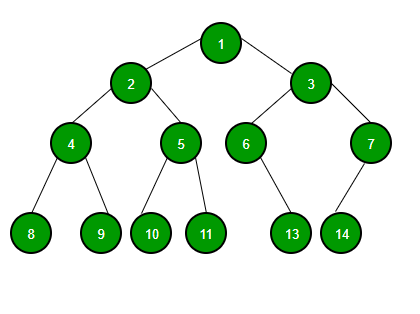
\includegraphics[scale=0.4]{img/binary_tree.png}
  \end{center}
\end{frame}

\begin{frame}
\frametitle{Grafo}
  \begin{center}
	  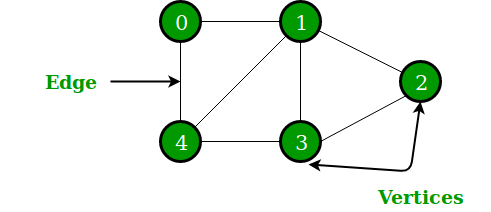
\includegraphics[scale=0.4]{img/graph.png}
  \end{center}
\end{frame}


\section{Bases de datos}
\begin{frame}
    \frametitle{bases de datos relacionales (SQLite, MySQL)}
    \pause
    \begin{itemize}
    \item Una base de datos relacional se refiere a un objeto digital donde se almacenan datos de una manera tabular en diferentes tablas. Dichas tablas pueden tener relación entre sí. Cada tabla consiste en sets de datos en columnas e hileras. 
    \end{itemize}
\end{frame}

\begin{frame}
  \begin{center}
	  \includegraphics[scale=0.4]{img/data_base_img.png}
  \end{center}
\end{frame}

\begin{frame} [fragile]
    \frametitle{Crear conexión e interactuar con una base de datos (MySQL)}
    \begin{itemize}
    \item Para poderse conectar a una base de datos con Python, es necesario tener la librería adecuada para el tipo de base de datos que deseamos.
    \item Por ejemplo, si deseamos conectarnos a una base de datos como MySQL, podemos hacer uso de la librería llamada mysql-connector-python
    \item Para instalarlo podemos correr el comando
    \end{itemize}
    \begin{lstlisting}[language=bash]
    $ pip install mysql-connector-python
    \end{lstlisting}
    o
    \begin{lstlisting}[language=bash]
    $ conda install mysql-connector-python
    \end{lstlisting}
\end{frame}

\begin{frame} [fragile]
    \begin{itemize}
    \item Una vez instalada la librería, es necesario importarla en nuestro script
    \end{itemize}
    \begin{lstlisting}[language=python]
    >> import mysql.connector
    >> from mysql.connector import Error
    \end{lstlisting}
\end{frame}

\begin{frame}
    \begin{itemize}
    \item Para crear una conexión se requiere conocer en donde se encuentra alojada la base de datos (host), el nombre de la base de datos a la que queremos acceder (database), el nombre del usuario con el que podemos acceder (use) y por último, la contraseña para dicho usuario (password)
    \pause
    \item En el siguiente bloque de código se intenta crear una conexión a una base de datos local (en nuestro equipo), en el caso que no se logre la conexión, el bloque try, except, finally, lanzará una excepción con el error que se originó al hacer la conexión.
    \end{itemize}
\end{frame}

\begin{frame}
    \begin{itemize}
    \item Si se logra hacer la conexión (se revisa con el método is\textunderscore connected() del objeto connection), buscamos la información del servidor (con el método get\textunderscore server\textunderscore info()), imprimimos dicha información y posteriormente se crea un cursor.
    \pause
    \item Un cursor es un puntero que nos permite interactuar con la base de datos.
    \item Al ejecutar una función, el cursor es quien le indica a la base de datos lo que va a hacer.
    \pause
    \item En nuestro caso, utilizamos el cursor para ejecutar el comando “select database();” con la función execute.
    \end{itemize}
\end{frame}

\begin{frame}
    \begin{itemize}
    \item Al hacer esto, la base de datos intentará ejecutar los comandos solicitados y los mantendrá en memoria hasta que sean traídos al ambiente de Python.
    \pause
    \item Para sacar dicha información podemos hacerlo a través de la función fetchone() o fetchall(). fetchone() iterará cada registro hasta agotar los resultados de la búsqueda, mientras que fetchall() traerá una lista completa con todos los registros.
    \end{itemize}
\end{frame}

\begin{frame}
    \begin{itemize}
    \item En el caso de este script, se seleccionó el nombre de la base de datos a la que se encuentra conectado.
    \pause
    \item Finalmente, revisamos si existe una conexión, y en caso de que así sea, cerramos el cursor y la conexión.
    \end{itemize}
\end{frame}

\begin{frame} [fragile]
    \begin{itemize}
    \item (con formato)
    \end{itemize}
    \begin{lstlisting}[basicstyle=\tiny][language=python]
    try:
    connection=mysql.connector.connect(host='localhost',
                                         database=prueba,
                                         user='root',
                                         password='')
    if connection.is_connected():
        db_Info = connection.get_server_info()
        print("Connected to MySQL Server version ", db_Info)
        cursor = connection.cursor()
        cursor.execute("select database();")
        record = cursor.fetchone()
        print("You're connected to database: ", record)
    except Error as e:
        print("Error while connecting to MySQL", e)
    finally:
    if (connection.is_connected()):
        cursor.close()
        connection.close()
        print("MySQL connection is closed")
    \end{lstlisting}
\end{frame}

\begin{frame} 
    \frametitle{Crear conexión e interactuar con una base de datos (Sqlite3)}
    \begin{itemize}
    \item Una base de datos Sqlite, en contraste a otras como MySQL, no trabaja sobre un motor de servidor-cliente. Esta base de datos se encuentra contenida en un archivo ordinario, por lo cual tiene limitantes.
    \item A diferencia también de otras bases de datos, esta no requiere parámetros como usuario y contraseña. Para trabajar con esta, es necesario saber dónde se encuentra el archivo y conectarse a él.
    \end{itemize}
\end{frame}

\begin{frame} [fragile]
    \begin{lstlisting}[basicstyle=\tiny][language=python]
try:
    conn = sqlite3.connect('db_sqlite.db')
    cursor = conn.cursor()
    print("Conectado a BD")
except sqlite3.Error as Error:
    print(error)
finally:
    if (conn):
        conn.close()
>>> 347

    \end{lstlisting}
\end{frame}

\begin{frame} [fragile]
    \frametitle{Seleccionando información}
    \begin{itemize}
    \item Ambas bases de datos manejan un lenguaje similar llamado SQL (Structured Query Language) o Lenguaje de Consulta Estructurado.
Para seleccionar información de una base de datos es necesario conocer la tabla de la cual queremos buscar información.
Si quisiéramos seleccionar todos los registros de una tabla de albums, ejecutamos con un cursor el comando y hacemos un fetchall():
    \end{itemize}
    \begin{lstlisting}[basicstyle=\tiny][language=python]
query = "SELECT * FROM albums;"
cursor.execute(query)
records = cursor.fetchall()
print(records)
>>> (1, 'For Those About To Rock We Salute You', 1)
>>> (2, 'Balls to the Wall', 2)
>>> (3, 'Restless and Wild', 2)
>>> (4, 'Let There Be Rock', 1)
>>> (5, 'Big Ones', 3)
...
    \end{lstlisting}
\end{frame}

\begin{frame} [fragile]
    \begin{itemize}
    \item Si queremos sólo ciertas columnas, podemos especificarlas en el SELECT
    \end{itemize}
    \begin{lstlisting}[basicstyle=\tiny][language=python]
query = "SELECT title FROM albums;"
cursor.execute(query)
records = cursor.fetchall()
print(records)
>>> ('For Those About To Rock We Salute You',)
>>> ('Balls to the Wall',)
>>> ('Restless and Wild',)
>>> ('Let There Be Rock',)
>>> ('Big Ones',)
    \end{lstlisting}
\end{frame}

\begin{frame} [fragile]
    \begin{itemize}
    \item Existe una cláusula que podemos utilizar para filtrar información, WHERE o dónde, nos permite especificar si queremos que una búsqueda contenga condiciones dentro de la información de sus columnas.
    \end{itemize}
    \begin{lstlisting}[basicstyle=\tiny][language=python]
query = "SELECT title, artistId FROM albums WHERE artistId > 10 and artistId < 20;"
cursor.execute(query)
records = cursor.fetchall()
print(records)
[ ('Alcohol Fueled Brewtality Live! [Disc 1]', 11)
('Alcohol Fueled Brewtality Live! [Disc 2]', 11)
('Black Sabbath', 12)
('Black Sabbath Vol. 4 (Remaster)', 12)
('Body Count', 13) ]
    \end{lstlisting}
\end{frame}

\begin{frame} [fragile]
    \frametitle{Procesando información con Python}
    \begin{itemize}
    \item Al ejecutar la función execute() sobre un cursor, podemos obtener las hileras de datos en un solo objeto a través de fetchall(), esto nos regresará una lista con tuplas que representan los datos de cada hilera.
    \end{itemize}
    \begin{lstlisting}[basicstyle=\tiny][language=python]
query = "SELECT title, artistId FROM albums WHERE artistId > 10 and artistId < 20;"
cursor.execute(query)
records = cursor.fetchall()
print(records)
[ ('Alcohol Fueled Brewtality Live! [Disc 1]', 11)
('Alcohol Fueled Brewtality Live! [Disc 2]', 11)
('Black Sabbath', 12)
('Black Sabbath Vol. 4 (Remaster)', 12)
('Body Count', 13) ]
    \end{lstlisting}
\end{frame}

\begin{frame} [fragile]
    \begin{itemize}
    \item Si queremos iterar cada hilera, podemos usar un bucle tipo for:
    \end{itemize}
    \begin{lstlisting}[basicstyle=\tiny][language=python]
for album in records:
    print(album)
>>> ('Alcohol Fueled Brewtality Live! [Disc 1]', 11)
>>> ('Alcohol Fueled Brewtality Live! [Disc 2]', 11)
>>> ('Black Sabbath', 12)
>>> ('Black Sabbath Vol. 4 (Remaster)', 12)
>>> ('Body Count', 13)
    \end{lstlisting}
\end{frame}

\begin{frame} [fragile]
    \begin{itemize}
    \item Otra forma de obtener los registros e iterarlos es través de la función fetchone()
    \end{itemize}
    \begin{lstlisting}[basicstyle=\tiny][language=python]
album = cursor.fetchone()
while album is not None:
    print(album)
    album = cursor.fetchone()
>>> ('Alcohol Fueled Brewtality Live! [Disc 1]', 11)
>>> ('Alcohol Fueled Brewtality Live! [Disc 2]', 11)
>>> ('Black Sabbath', 12)
>>> ('Black Sabbath Vol. 4 (Remaster)', 12)
>>> ('Body Count', 13)
    \end{lstlisting}
\end{frame}

\begin{frame} [fragile]
    \frametitle{Juntando tablas relacionadas}
    \begin{itemize}
    \item Para juntar tablas que tienen relación entre si, podemos usar la función JOIN, y especificamos las columnas que se encuentran relacionadas.
    \end{itemize}
    \begin{lstlisting}[basicstyle=\tiny][language=python]
query = "SELECT albums.Title, artists.Name FROM albums LEFT JOIN artists on (albums.ArtistId = artists.ArtistId);"
cursor.execute(query)
records = cursor.fetchall()
for record in records:
        print(record)
>>> ('For Those About To Rock We Salute You', 'AC/DC')
>>> ('Balls to the Wall', 'Accept')
>>> ('Restless and Wild', 'Accept')
>>> ('Let There Be Rock', 'AC/DC')
>>> ('Big Ones', 'Aerosmith')

    \end{lstlisting}
\end{frame}





\section{Introducción a Numpy}
\begin{frame} [fragile]
    \frametitle{Instalando e Importando NumPy}
    \pause
    \begin{itemize}
    \item Numpy es una librería que nos permite trabajar con datos de una manera muy eficiente y rápida.
    \end{itemize}
    
    \begin{lstlisting}[language=bash]
    $pip install numpy, o conda install numpy
    \end{lstlisting}
    \begin{lstlisting}[language=python]
    import numpy as np
    \end{lstlisting}
\end{frame}

\begin{frame} [fragile]
    \frametitle{Creando arreglos y matrices}
    \begin{itemize}
    \item Crear arreglo de np de una lista de Python
    \end{itemize}
    \begin{lstlisting}[basicstyle=\tiny][language=python]
lista = [1, 2, 3, 4, 5]
lista_np = np.array(lista)
>>> array([1, 2, 3, 4, 5])
    \end{lstlisting}
    
    \begin{itemize}
    \item Con valores inicializados en 0 (np.zeros())
    \end{itemize}
    \begin{lstlisting}[basicstyle=\tiny][language=python]
np_lista_zeros = np.zeros(10)
np_lista_zeros
>>> array([0., 0., 0., 0., 0., 0., 0., 0., 0., 0.])
    \end{lstlisting}
\end{frame}

\begin{frame} [fragile]
    \frametitle{Creando arreglos}
    
    \begin{itemize}
    \item Con valores inicializados en 1 (np.ones())
    \end{itemize}
    \begin{lstlisting}[basicstyle=\tiny][language=python]
np_lista_ones = np.ones(10)
np_lista_ones
>>> array([1., 1., 1., 1., 1., 1., 1., 1., 1., 1.])
    \end{lstlisting}
    
    \begin{itemize}
    \item Definiendo un comienzo, fin y la cantidad de elementos (np.linspace())
    \end{itemize}
    \begin{lstlisting}[basicstyle=\tiny][language=python]
np_linspace = np.linspace(1, 10)
print(len(np_linspace))
>>> 50
np_linspace = np.linspace(1, 10, 10)
print(np_linspace)
>>> [ 1.  2.  3.  4.  5.  6.  7.  8.  9. 10.]
    \end{lstlisting}
\end{frame}

\begin{frame} [fragile]
    \frametitle{Creando arreglos}
    \begin{itemize}
    \item Con valores aleatorios (np.random.randint())
    \end{itemize}
    \begin{lstlisting}[basicstyle=\tiny][language=python]
np_random = np.random.randint(10, size=10)
np_random
>>> array([7, 8, 4, 3, 4, 7, 7, 2, 6, 2])
np_random = np.random.randint(10, 20, size=10)
np_random
>>> array([15, 11, 17, 16, 19, 16, 19, 10, 19, 19])
    \end{lstlisting}

\end{frame}

\begin{frame}
    \frametitle{Creando matrices}
    \begin{itemize}
    \item Para crear matrices de 2 o más dimensiones usamos la función deseada para los valores default (zeros(), ones(), etc), y en vez de pasar el número de elementos que queremos, pasamos una tupla especificando la forma que queremos.
    \item Para una matriz de 2 dimensiones pasamos (x, y), para una de 3 pasamos (x, y, z), para más niveles (x, y… n)
    \end{itemize}
\end{frame}

\begin{frame} [fragile]
    \frametitle{Creando matrices}
    \begin{lstlisting}[basicstyle=\tiny][language=python]
np.zeros((4, 4))
>>> array([[0., 0., 0., 0.],
       [0., 0., 0., 0.],
       [0., 0., 0., 0.],
       [0., 0., 0., 0.]])
np.zeros((3, 3, 3))
>>> array([[[0., 0., 0.],
        [0., 0., 0.],
        [0., 0., 0.]],

       [[0., 0., 0.],
        [0., 0., 0.],
        [0., 0., 0.]],

       [[0., 0., 0.],
        [0., 0., 0.],
        [0., 0., 0.]]])
    \end{lstlisting}
\end{frame}

\begin{frame} [fragile]
    \frametitle{Manipulación y operaciones en arreglos}
    \begin{itemize}
    \item Cómo obtener secciones de arreglos
    \end{itemize}
    \begin{lstlisting}[basicstyle=\tiny][language=python]
lista = [1, 2, 3, 4, 5]
lista_np = np.array(lista)
>>> array([1, 2, 3, 4, 5])
print(lista_np[0])
>>> 1
print(lista_np[0:2])
>>> [1, 2]
print(lista_np[:4])
>>> [1, 2, 3, 4]
print(lista_np[-1]
>>> 5
print(np.where(lista_np > 2))
>>> [1, 2, 3, 4] # regresa el index
nueva_lista = lista_np[np.where(lista_np > 2)]
print(nueva_lista)
>>> [3, 4, 5]
    \end{lstlisting}
\end{frame}

\begin{frame} [fragile]
    \frametitle{Manipulación y operaciones en arreglos}
    \begin{itemize}
    \item Operaciones y funciones de arreglos
    \end{itemize}
    \begin{lstlisting}[basicstyle=\tiny][language=python]
np.sum(lista_np)
>>> 15
np.prod(lista_np)
>>> 120
np.mean(lista_np)
>>> 3
np.std(lista_np)
>>> 1.4142135623730951
np.var(lista_np)
>>> 2.0
np.min(lista_np)
>>> 1
np.max(lista_np)
>>> 5

lista_np + lista_np
>>> [2,  4,  6,  8, 10]
lista_np + 30
>>> [31, 32, 33, 34, 35]
lista_np * lista_np
>>> [ 1,  4,  9, 16, 25]
    \end{lstlisting}
\end{frame}

\begin{frame} [fragile]
    \frametitle{Manipulación y operaciones en arreglos}
    \begin{itemize}
    \item Operaciones con np.where()
    \end{itemize}
    \begin{lstlisting}[basicstyle=\tiny][language=python]
np.where(lista_np > 2, 10, lista_np)
>>> [ 1,  2, 10, 10, 10]
np.where(lista_np > 2, 10, 0)
>>> [ 0,  0, 10, 10, 10]
    \end{lstlisting}
\end{frame}

\begin{frame} [fragile]
    \frametitle{Manipulación y operaciones en arreglos}
    \begin{itemize}
    \item Cambiar la figura/aspecto del arreglo (np.shape(), np.reshape(), np.flatten())
    \end{itemize}
    \begin{lstlisting}[basicstyle=\tiny][language=python]
lista_np2 = np.array([1,2,3,4,5,6,7,8,9,10])
lista_np2.shape = (5,2)
print(lista_np2)
>>> [[ 1  2]
 [ 3  4]
 [ 5  6]
 [ 7  8]
 [ 9 10]]
lista_np2.shape = (2, 5)
print(lista_np2)
>>> [[ 1  2  3  4  5]
 [ 6  7  8  9 10]]
print(lista_np2.flatten())
>>> [ 1  2  3  4  5  6  7  8  9 10]
    \end{lstlisting}
\end{frame}


\section{Ejercicios (Día 2)}
\begin{frame}
    \frametitle{Ejercicios}
    \pause
    \begin{itemize}
    \item Escribe un programa que regrese un string hecho por los primeros 2 y los últimos 2 caracteres de un string dado. Si la longitud del string es menor a 2, regresar un string vacío. (ejemplo: Entradag : 'python3'
    Salida: 'pyn3'
    \item Dado un string, crear una función que cuente la ocurrencia de cada letra dentro del string
    \item Implementar una función sumatoria de 2i+1 donde tenemos una lista de valores numéricos, los cuales multiplicaremos cada valor por 2, seguido le sumaremos un 1 a cada valor, y finalmente sumaremos todos los valores de la lista
	lista = [1, 2, 3 ,4]
	Resultado = 24
	\item Escribe un programa que remueva los duplicados de un diccionario
	\item Escribe un programa que escriba en un archivo los valores de un diccionario separando la llave de su valor en diferentes columnas
	\item Escribe un programa que calcule el determinante de un arreglo
    \end{itemize}
\end{frame}


\begin{frame}[fragile]{Code}
    \frametitle{Ejercicios}
    \pause
    \begin{itemize}
    \item Crear una función que se conecte al archivo de sqlite, buscar todos los albums y juntarlos con la tabla de artists. Iterar todos los registros y crear un diccionario donde la llave será el nombre del artista y su contenido será un arreglo con la lista de sus albums
    \end{itemize}
    
  \begin{block}{ejemplo:} % alertblock, exampleblock
	  \begin{lstlisting}
{
    `AC/DC': [
    `For those about to Rock we salute You',
    `Let There Be Rock'
    ],
`Accept': []
}


	  \end{lstlisting}
  \end{block}
    
\end{frame}


\section{Bibliografía}
\begin{frame}[fragile]
  \frametitle{Referencias}
  \begin{itemize}
	\item (=
	\pause
  \end{itemize}

    \begin{block}{Bibliografías} % alertblock, exampleblock
	  \begin{lstlisting}
https://www.tutorialspoint.com/python/python_basic_operators.htm
https://www.tutorialsteacher.com/python/python-comparison-and-logical-operators
https://www.learnpython.org/es/Hello,%20World!
https://www.w3schools.com/python/python_lists.asp
https://www.guru99.com/reading-and-writing-files-in-python.html
https://www.tutorialpython.com/modulos-python/
https://www.tutorialspoint.com/python_data_structure/python_binary_tree.htm
	  \end{lstlisting}
  \end{block}
  
\end{frame}

\end{document}


